
\de{ĐỀ THI GIỮA HỌC KỲ II NĂM HỌC 2022-2023}{THCS-THPT Diên Hồng}


\begin{bt}%[0T7Y1-1]%[Dự án đề kiểm tra HKII NH22-23- Tên GV]%[THCS-THPT Diên Hồng]
	Xét dấu tam thức bậc hai sau $f(x) =2x^2+4x-6$.
\loigiai{
Phương trình $f(x)=0$ có hai nghiệm phân biệt là $x=1$ và $x=-3$.\\
Bảng xét dấu
\begin{center}

\begin{tikzpicture}
	\tkzTabInit[lgt=3]	%lgt độ rộng cột x,f(x);espcl độ rộng của cột
	{$x$/1,$f(x)$/1}
	{$-\infty$,$-3$,$1$,$+\infty$}
	\tkzTabLine{,+,0,-,0,+,}
\end{tikzpicture}
\end{center}
Vậy $f(x)>0$ trên khoảng $(-\infty;-3)$ và $(1;+\infty)$.\\
$f(x)<0$ trên khoảng $(-3;1)$.
}
\end{bt}
\begin{bt}%[0T7Y2-1]%[0T7B2-1]%[Dự án đề kiểm tra HKII NH22-23- Tên GV]%[THCS-THPT Diên Hồng]
	Giải các bất phương trình bậc hai sau
	\begin{enumerate}
		\item $-5x^2+4x+12>0$.
		\item $(x+1)^2\leq 2x^2-x+3$.
	\end{enumerate}
\loigiai{
\begin{enumerate}
	\item Bảng xét dấu
	\begin{center}
		\begin{tikzpicture}
			\tkzTabInit[lgt=4]	%lgt độ rộng cột x,f(x);espcl độ rộng của cột
			{$x$/1,$-5x^2+4x+12$/1}
			{$-\infty$,$-\dfrac{6}{5}$,$2$,$+\infty$}
			\tkzTabLine{,-,0,+,0,-,}
		\end{tikzpicture}
	\end{center}
	Vậy tập nghiệm của bất phương trình là $S=\left(-\dfrac{6}{5};2\right)$.
	\item Ta có
	\begin{equation*}
		(x+1)^2\leq 2x^2-x+3\Leftrightarrow x^2-3x+2\geq 0.
	\end{equation*}
	Bảng xét dấu
	\begin{center}
		
\begin{tikzpicture}
			\tkzTabInit[lgt=4]	%lgt độ rộng cột x,f(x);espcl độ rộng của cột
			{$x$/1,$x^2-3x+2$/1}
			{$-\infty$,$1$,$2$,$+\infty$}
			\tkzTabLine{,+,0,-,0,+,}
		\end{tikzpicture}
	\end{center}
	Vậy tập nghiệm của bất phương trình là $S=\left(-\infty;1\right]\cup\left[2;+\infty\right)$.
\end{enumerate}
}
\end{bt}
\begin{bt}%[0T7Y2-1]%[0T7Y2-1]%[Dự án đề kiểm tra HKII NH22-23- Tên GV]%[THCS-THPT Diên Hồng]
	Lợi nhuận $(I)$ từ tiền bán vé mỗi ngày của một rạp chiếu phim phụ thuộc vào giá vé $(x)$ của ngày hôm đó theo công thức $I = -37x^2 + 4500x- 120000$, với $I$ và $x$ được tính bằng nghìn đồng.
	\begin{enumerate}
		\item Tìm mức vé sao cho ngày hôm đó rạp phim có lãi.
		\item Nếu mức vé là $100$ nghìn đồng thì ngày hôm đó rạp phim có lãi không? Vì sao?
	\end{enumerate}
	\loigiai{
		Ta có
		\begin{equation*}
			-37x^2 + 4500x- 120000 = 0\Leftrightarrow \hoac{&x\approx 82\\&x\approx39.}
		\end{equation*}
		Bảng xét dấu
		\begin{center}
			
\begin{tikzpicture}
				\tkzTabInit[lgt=4]	%lgt độ rộng cột x,f(x);espcl độ rộng của cột
				{$x$/1,$I$/1}
				{$-\infty$,$39$,$82$,$+\infty$}
				\tkzTabLine{,-,0,+,0,-,}
			\end{tikzpicture}
		\end{center}
		Để rạp phim có lãi thì lợi nhuận lớn hơn $0$, nghĩa là $I(x)>0$
		\begin{enumerate}
			\item Mức vé để ngày hôm đó rạp phim có lãi là từ $39$ nghìn đồng đến $82$ nghìn đồng.
			\item Mức vé để rạp chiếu phim không có lãi là nhỏ hơn $39$ nghìn và lớn hơn $82$ nghìn.\\
			Vậy nếu mức vé là $100$ nghìn đồng thì ngày hôm đó rạp phim không có lãi.
		\end{enumerate}
	}
\end{bt}


\begin{bt}%[0T7K1-1]%[Dự án đề kiểm tra GKII NH22-23- Hieu Phan]%[THCS-THPT DIÊN HỒNG]
Cho tam thức bậc hai $ f(x)=(m-1)x^2-(m-1)x+2m+1 $. Xác định $ m $ để $ f(x)\ge 0, \forall x \in \mathbb{R} $.
\loigiai{
    \begin{itemize}
        \item Xét $m=1$, khi đó $f(x)=3>0 \forall x \in \mathbb{R}$.
        \item Xét $m\ne 1$, khi đó \\
        $ f(x)\ge 0, \forall x \in \mathbb{R} $ khi và chỉ khi
        \begin{eqnarray*}
            \heva{&a>0 \\ & \Delta \le 0}&\Leftrightarrow& \heva{& m>1 \\ & (m-1)^2-4(m-1)(2m+1)\le 0 }\\
            &\Leftrightarrow& \heva{& m>1 \\ &-7m^2 +2m+5\le 0}\Leftrightarrow  \heva{& m>1 \\ &\hoac{& m\le -\dfrac{5}{7} \\ &  m\ge 1}}\Leftrightarrow m>1. 
        \end{eqnarray*}
    \end{itemize}
Vậy $m\ge 1$ thì $ f(x)\ge 0, \forall x \in \mathbb{R} $.
}
\end{bt}
\begin{bt}%[0T7K3-2]%[Dự án đề kiểm tra GKII NH22-23- Hieu Phan]%[THCS-THPT DIÊN HỒNG]
Giải phương trình $ \sqrt{4+2x-x^2}=x-2 $.
\loigiai{
    Ta có  \begin{eqnarray*}
        \sqrt{4+2x-x^2}=x-2& \Rightarrow& 4+2x-x^2=(x-2)^2\\
                                               &\Leftrightarrow& 2x^2-6x=0 \Leftrightarrow \hoac{& x=0 \\ & x=3. }
    \end{eqnarray*}
Thế $ x=3 $ và $ x=0 $ vào phương trình đã cho ta thấy $ x=3 $ là nghiệm của phương trình.
}
\end{bt}
\begin{bt}%[0T9K2-2]%[Dự án đề kiểm tra GKII NH22-23- Hieu Phan]%[THCS-THPT DIÊN HỒNG]
 Trong mặt phẳng $ Oxy $, cho tam giác $ ABC $ có tọa độ các đỉnh là $ A(2;5),B(1;2) $ và $ C(4;-7) $.

 \begin{enumerate}
     \item Tìm tọa độ điểm $ D $ để $ ABCD $ là hình bình hành. Tìm tọa độ của tâm hình bình hành đó.
     \item Tìm tọa độ chân đường cao $ H $ vẽ từ $ A $ của tam giác $ ABC $.
     \item Viết phương trình đường thẳng $ AC $ và phương trình đường cao $ BK $ của tam giác $ ABC$.
     \item Gọi $ G $ là trọng tâm của tam giác $ ABC $. Tìm tọa độ điểm $ G $ và tính khoảng cách từ $ G $ đến đường thẳng $ \Delta\colon 3x+y-3=0 $.
 \end{enumerate}
    \loigiai{
     \begin{enumerate}
        \item Gọi $ D(x;y) $.  $ ABCD $ là hình bình hành khi 
        $$\vec{AB}=\vec{DC}\Leftrightarrow \heva{& 4-x=-1 \\ & -7-y=-3}\Leftrightarrow \heva{&x=5 \\ &y=-4. }  $$
        Vậy $ D(5;-4) $.\\
        Gọi $O(x;y)$ là tâm của hình bình hành. Khi đó $O$ là trung điểm của $AC$.\\
        Suy ra $\heva{&x=\dfrac{2+4}{2} \\ &y=\dfrac{5-7}{2} }\Leftrightarrow \heva{& x=3 \\ &y=-1. }$\\
        Vậy $O(3;-1)$.
        \item Gọi $ H(x_H;y_H) $. Ta có $\vec{BC}=(3;-9)$.\\
        Phương trình đường thẳng $BC\colon \dfrac{x-1}{3}=\dfrac{y-2}{-9}\Leftrightarrow 3x+y-5=0$.\\
        $H$ là chân đường cao vẽ từ $ A $ của tam giác $ ABC $ nên
        $$\heva{& \vec{AH}\perp \vec{BC} \\ & H \in BC }\Leftrightarrow \heva{& 3(x_H-2) -9(y_H-5)=0\\ & y_H=5-3x_H}\Leftrightarrow \heva{& x_H=\dfrac{1}{5} \\ & y_H=\dfrac{22}{5}.}$$
        Vậy $ H\left(\dfrac{1}{5};\dfrac{22}{5}\right) $.
        \item Ta có $\vec{AC}=(2;-12)$.\\
        Phương trình đường thẳng $ AC \colon \dfrac{x-2}{2}=\dfrac{y-5}{-12}\Leftrightarrow 6x+y-17=0$.\\
        Phương trình đường cao $ BK\colon 2(x-1) -12(y-2)=0\Leftrightarrow x-6y+11=0$.
        \item $ G $ là trọng tâm của tam giác $ ABC $ nên ta có
        $$\heva{&x_G= \dfrac{2+1+4}{3}=\dfrac{7}{3} \\ &y_G=\dfrac{5+2-7}{3}=0 }\Rightarrow G\left(\dfrac{7}{3};0 \right).$$
        Ta có $\mathrm{d}(G;\Delta)=\dfrac{\bigg|3\cdot \dfrac{7}{3}+0-3\bigg|}{\sqrt{3^2+1}}=\dfrac{2\sqrt{10}}{5}$.
    \end{enumerate}
}
\end{bt}